% Options for packages loaded elsewhere
\PassOptionsToPackage{unicode}{hyperref}
\PassOptionsToPackage{hyphens}{url}
%
\documentclass[
  english,
  man]{apa6}
\title{EDLD 640 Capstone}
\author{Diana DeWald\textsuperscript{1} \& Dare Baldwin\textsuperscript{1}}
\date{}

\usepackage{amsmath,amssymb}
\usepackage{lmodern}
\usepackage{iftex}
\ifPDFTeX
  \usepackage[T1]{fontenc}
  \usepackage[utf8]{inputenc}
  \usepackage{textcomp} % provide euro and other symbols
\else % if luatex or xetex
  \usepackage{unicode-math}
  \defaultfontfeatures{Scale=MatchLowercase}
  \defaultfontfeatures[\rmfamily]{Ligatures=TeX,Scale=1}
\fi
% Use upquote if available, for straight quotes in verbatim environments
\IfFileExists{upquote.sty}{\usepackage{upquote}}{}
\IfFileExists{microtype.sty}{% use microtype if available
  \usepackage[]{microtype}
  \UseMicrotypeSet[protrusion]{basicmath} % disable protrusion for tt fonts
}{}
\makeatletter
\@ifundefined{KOMAClassName}{% if non-KOMA class
  \IfFileExists{parskip.sty}{%
    \usepackage{parskip}
  }{% else
    \setlength{\parindent}{0pt}
    \setlength{\parskip}{6pt plus 2pt minus 1pt}}
}{% if KOMA class
  \KOMAoptions{parskip=half}}
\makeatother
\usepackage{xcolor}
\IfFileExists{xurl.sty}{\usepackage{xurl}}{} % add URL line breaks if available
\IfFileExists{bookmark.sty}{\usepackage{bookmark}}{\usepackage{hyperref}}
\hypersetup{
  pdftitle={EDLD 640 Capstone},
  pdfauthor={Diana DeWald1 \& Dare Baldwin1},
  pdflang={en-EN},
  pdfkeywords={causal learning models, pedagogy, text analysis},
  hidelinks,
  pdfcreator={LaTeX via pandoc}}
\urlstyle{same} % disable monospaced font for URLs
\usepackage{color}
\usepackage{fancyvrb}
\newcommand{\VerbBar}{|}
\newcommand{\VERB}{\Verb[commandchars=\\\{\}]}
\DefineVerbatimEnvironment{Highlighting}{Verbatim}{commandchars=\\\{\}}
% Add ',fontsize=\small' for more characters per line
\usepackage{framed}
\definecolor{shadecolor}{RGB}{248,248,248}
\newenvironment{Shaded}{\begin{snugshade}}{\end{snugshade}}
\newcommand{\AlertTok}[1]{\textcolor[rgb]{0.94,0.16,0.16}{#1}}
\newcommand{\AnnotationTok}[1]{\textcolor[rgb]{0.56,0.35,0.01}{\textbf{\textit{#1}}}}
\newcommand{\AttributeTok}[1]{\textcolor[rgb]{0.77,0.63,0.00}{#1}}
\newcommand{\BaseNTok}[1]{\textcolor[rgb]{0.00,0.00,0.81}{#1}}
\newcommand{\BuiltInTok}[1]{#1}
\newcommand{\CharTok}[1]{\textcolor[rgb]{0.31,0.60,0.02}{#1}}
\newcommand{\CommentTok}[1]{\textcolor[rgb]{0.56,0.35,0.01}{\textit{#1}}}
\newcommand{\CommentVarTok}[1]{\textcolor[rgb]{0.56,0.35,0.01}{\textbf{\textit{#1}}}}
\newcommand{\ConstantTok}[1]{\textcolor[rgb]{0.00,0.00,0.00}{#1}}
\newcommand{\ControlFlowTok}[1]{\textcolor[rgb]{0.13,0.29,0.53}{\textbf{#1}}}
\newcommand{\DataTypeTok}[1]{\textcolor[rgb]{0.13,0.29,0.53}{#1}}
\newcommand{\DecValTok}[1]{\textcolor[rgb]{0.00,0.00,0.81}{#1}}
\newcommand{\DocumentationTok}[1]{\textcolor[rgb]{0.56,0.35,0.01}{\textbf{\textit{#1}}}}
\newcommand{\ErrorTok}[1]{\textcolor[rgb]{0.64,0.00,0.00}{\textbf{#1}}}
\newcommand{\ExtensionTok}[1]{#1}
\newcommand{\FloatTok}[1]{\textcolor[rgb]{0.00,0.00,0.81}{#1}}
\newcommand{\FunctionTok}[1]{\textcolor[rgb]{0.00,0.00,0.00}{#1}}
\newcommand{\ImportTok}[1]{#1}
\newcommand{\InformationTok}[1]{\textcolor[rgb]{0.56,0.35,0.01}{\textbf{\textit{#1}}}}
\newcommand{\KeywordTok}[1]{\textcolor[rgb]{0.13,0.29,0.53}{\textbf{#1}}}
\newcommand{\NormalTok}[1]{#1}
\newcommand{\OperatorTok}[1]{\textcolor[rgb]{0.81,0.36,0.00}{\textbf{#1}}}
\newcommand{\OtherTok}[1]{\textcolor[rgb]{0.56,0.35,0.01}{#1}}
\newcommand{\PreprocessorTok}[1]{\textcolor[rgb]{0.56,0.35,0.01}{\textit{#1}}}
\newcommand{\RegionMarkerTok}[1]{#1}
\newcommand{\SpecialCharTok}[1]{\textcolor[rgb]{0.00,0.00,0.00}{#1}}
\newcommand{\SpecialStringTok}[1]{\textcolor[rgb]{0.31,0.60,0.02}{#1}}
\newcommand{\StringTok}[1]{\textcolor[rgb]{0.31,0.60,0.02}{#1}}
\newcommand{\VariableTok}[1]{\textcolor[rgb]{0.00,0.00,0.00}{#1}}
\newcommand{\VerbatimStringTok}[1]{\textcolor[rgb]{0.31,0.60,0.02}{#1}}
\newcommand{\WarningTok}[1]{\textcolor[rgb]{0.56,0.35,0.01}{\textbf{\textit{#1}}}}
\usepackage{graphicx}
\makeatletter
\def\maxwidth{\ifdim\Gin@nat@width>\linewidth\linewidth\else\Gin@nat@width\fi}
\def\maxheight{\ifdim\Gin@nat@height>\textheight\textheight\else\Gin@nat@height\fi}
\makeatother
% Scale images if necessary, so that they will not overflow the page
% margins by default, and it is still possible to overwrite the defaults
% using explicit options in \includegraphics[width, height, ...]{}
\setkeys{Gin}{width=\maxwidth,height=\maxheight,keepaspectratio}
% Set default figure placement to htbp
\makeatletter
\def\fps@figure{htbp}
\makeatother
\setlength{\emergencystretch}{3em} % prevent overfull lines
\providecommand{\tightlist}{%
  \setlength{\itemsep}{0pt}\setlength{\parskip}{0pt}}
\setcounter{secnumdepth}{-\maxdimen} % remove section numbering
% Make \paragraph and \subparagraph free-standing
\ifx\paragraph\undefined\else
  \let\oldparagraph\paragraph
  \renewcommand{\paragraph}[1]{\oldparagraph{#1}\mbox{}}
\fi
\ifx\subparagraph\undefined\else
  \let\oldsubparagraph\subparagraph
  \renewcommand{\subparagraph}[1]{\oldsubparagraph{#1}\mbox{}}
\fi
\newlength{\cslhangindent}
\setlength{\cslhangindent}{1.5em}
\newlength{\csllabelwidth}
\setlength{\csllabelwidth}{3em}
\newlength{\cslentryspacingunit} % times entry-spacing
\setlength{\cslentryspacingunit}{\parskip}
\newenvironment{CSLReferences}[2] % #1 hanging-ident, #2 entry spacing
 {% don't indent paragraphs
  \setlength{\parindent}{0pt}
  % turn on hanging indent if param 1 is 1
  \ifodd #1
  \let\oldpar\par
  \def\par{\hangindent=\cslhangindent\oldpar}
  \fi
  % set entry spacing
  \setlength{\parskip}{#2\cslentryspacingunit}
 }%
 {}
\usepackage{calc}
\newcommand{\CSLBlock}[1]{#1\hfill\break}
\newcommand{\CSLLeftMargin}[1]{\parbox[t]{\csllabelwidth}{#1}}
\newcommand{\CSLRightInline}[1]{\parbox[t]{\linewidth - \csllabelwidth}{#1}\break}
\newcommand{\CSLIndent}[1]{\hspace{\cslhangindent}#1}
% Manuscript styling
\usepackage{upgreek}
\captionsetup{font=singlespacing,justification=justified}

% Table formatting
\usepackage{longtable}
\usepackage{lscape}
% \usepackage[counterclockwise]{rotating}   % Landscape page setup for large tables
\usepackage{multirow}		% Table styling
\usepackage{tabularx}		% Control Column width
\usepackage[flushleft]{threeparttable}	% Allows for three part tables with a specified notes section
\usepackage{threeparttablex}            % Lets threeparttable work with longtable

% Create new environments so endfloat can handle them
% \newenvironment{ltable}
%   {\begin{landscape}\centering\begin{threeparttable}}
%   {\end{threeparttable}\end{landscape}}
\newenvironment{lltable}{\begin{landscape}\centering\begin{ThreePartTable}}{\end{ThreePartTable}\end{landscape}}

% Enables adjusting longtable caption width to table width
% Solution found at http://golatex.de/longtable-mit-caption-so-breit-wie-die-tabelle-t15767.html
\makeatletter
\newcommand\LastLTentrywidth{1em}
\newlength\longtablewidth
\setlength{\longtablewidth}{1in}
\newcommand{\getlongtablewidth}{\begingroup \ifcsname LT@\roman{LT@tables}\endcsname \global\longtablewidth=0pt \renewcommand{\LT@entry}[2]{\global\advance\longtablewidth by ##2\relax\gdef\LastLTentrywidth{##2}}\@nameuse{LT@\roman{LT@tables}} \fi \endgroup}

% \setlength{\parindent}{0.5in}
% \setlength{\parskip}{0pt plus 0pt minus 0pt}

% \usepackage{etoolbox}
\makeatletter
\patchcmd{\HyOrg@maketitle}
  {\section{\normalfont\normalsize\abstractname}}
  {\section*{\normalfont\normalsize\abstractname}}
  {}{\typeout{Failed to patch abstract.}}
\patchcmd{\HyOrg@maketitle}
  {\section{\protect\normalfont{\@title}}}
  {\section*{\protect\normalfont{\@title}}}
  {}{\typeout{Failed to patch title.}}
\makeatother
\shorttitle{Natural Language Processing for Pedagogy}
\keywords{causal learning models, pedagogy, text analysis\newline\indent Word count: 2756}
\DeclareDelayedFloatFlavor{ThreePartTable}{table}
\DeclareDelayedFloatFlavor{lltable}{table}
\DeclareDelayedFloatFlavor*{longtable}{table}
\makeatletter
\renewcommand{\efloat@iwrite}[1]{\immediate\expandafter\protected@write\csname efloat@post#1\endcsname{}}
\makeatother
\usepackage{lineno}

\linenumbers
\usepackage{csquotes}
\ifXeTeX
  % Load polyglossia as late as possible: uses bidi with RTL langages (e.g. Hebrew, Arabic)
  \usepackage{polyglossia}
  \setmainlanguage[]{english}
\else
  \usepackage[main=english]{babel}
% get rid of language-specific shorthands (see #6817):
\let\LanguageShortHands\languageshorthands
\def\languageshorthands#1{}
\fi
\ifLuaTeX
  \usepackage{selnolig}  % disable illegal ligatures
\fi


\affiliation{\vspace{0.5cm}\textsuperscript{1} University of Oregon}

\abstract{
How is young children's exploration impacted by adult pedagogy? Can we create Machine Learning models to predict how a child will explore the causal features of an object based upon the pedagogy they are exposed to? Our goal is to establish predictive models of preschoolers' causal learning outcomes within educational settings based upon teachers' pedagogical styles. Using pre-existing samples of pedagogy and child outcomes, we created three machine learning models to capture 1) the extent to which adults produce pedagogy that is likely to have the intended effect on preschoolers' play behavior when prompted accordingly, and 2) the extent to which pedagogy that has different intent based upon the prompt differs in sentiment. We found that sentiment of pedagogical statements did not seem to be related to whether participants were in a condition to enhance or to constrain exploration. We also found that the number of unique actions a child performed had to do with their likelihood of discovering the squeaker target function (introduced in pedagogy).
}



\begin{document}
\maketitle

\hypertarget{introduction}{%
\section{Introduction}\label{introduction}}

Developmentalists and educators have long debated the benefits of child-directed (Montessori style) exploration contra adult-directed (pedagogical) instruction on learning outcomes. While young children (age 3-6) often re-structure their hypotheses about the world based upon self-directed exploration á la Montessori, there are many subjects children cannot master without adult-directed pedagogical guidance (e.g., novel object labels, the alphabet, color and shape labels, historical events, the existence of entities such as germs, etc.). Such subjects are often culturally and linguistically bound, but even causal learning related to the physical properties of objects and entities can benefit from adult-directed pedagogy. Clarifying the extent to which pedagogy supports---and in some cases diminishes---effective causal learning is essential for a) informing teaching strategies in a time when many preparatory schools in the U.S. suffer from a lack of funding and teacher support (\textbf{SRCD?}; \textbf{NIERR?}), and b) elevating early education outcomes following relative dips in school preparedness over the past three years (Jalongo, 2021; (\textbf{gonzalez2022school?})).
Those who have sought to address the impact of adult-directed pedagogy on causal learning describe a pedagogical trade-off model. This model proposes that adult instruction increases the proportion of time children spend exploring an object's pedagogy-relevant properties but limits their investigation of other properties. Conversely, child-directed exploration is understood to produce broader discovery of the complete set of an object's causal properties but diminish the time spent investigating any particular property.While such behavioral outcomes are established, little is known about the differential impact of diverse pedagogy types (such method tend to rely on one pedagogical condition statement, usually ``This is how my toy works'').
In this project, we were interested in the relation between adults' use of language while teaching and children's learning outcomes. Specifically, we wanted to investigate how diverse and naturalistic pedagogy types that were produced to encourage children's play based upon findings from the pedagogy trade-off model would align with the pedagogy utilized within typical empirical methods for this model. To examine this, we took pre-existing text data from a survey where we asked UO students to watch a video depicting a toy and generate a text response detailing how they would go about teaching a preschooler about the toy. In one between subjects condition, they were instructed to `enhance' exploration (i.e., by providing pedagogy that would encourage a child to explore beyond one object property). In a second condition, they were instructed to `constrain exploration (i.e., by providing pedagogy that would encourage a child to only explore the one property demonstrated in the video).
After presenting descriptives on the survey text dataset, we go on to describe three machine learning models to investigate different aims. The first model was created to predict the likelihood of a positive or negative sentiment occurring based upon the condition (enhance or constrain), source (qualtrics survey or pre-existing study pedagogy) and function (we included both a 'squeaker' and a `light' function in the object introduction video). The second model was created to predict the distance among expected outcomes paired via a manual coding system to the pedagogy samples from the survey (K-nearest neighbors). The third model again used logistic regression to create a best-performing model predicting child play outcomes (we collected in Fall of 2022 at the Oregon Museum of Science and Industry) from 4 pedagogy types used in that method.

\hypertarget{methods}{%
\section{Methods}\label{methods}}

\begin{verbatim}
In Fall of 2022, we conducted a Qualtrics survey of undergraduate students 
\end{verbatim}

(N = 168) at the University of Oregon, asking participants to report how they
would teach a child about the causal properties of a novel object. Participants
were randomly sorted into 2 conditions. In the `enhance' condition, participants
were instructed to generate pedagogy for two object properties with the intention
to produce broad exploratory behaviors from a child (prompt: ``what would you say )
to intoduce this toy in a way that encourages wide-ranging exploration?''). In the
`constrain' condition, participants were asked to generate pedagogy intended to
produce limited exploratory behaviors from a child (prompt: ``What would you say )
to introduce this toy in a way that discourages wide-ranging exploration?''). We
subsequently assessed overall word frequencies, and word frequencies by condition
(see `Results: Descriptive Plots'). Next, we investigated the extent to which the
`constrain' pedagogy differed in sentiment from the `enhance' pedagogy (see\\
`Results: Model 1')
In Model 2, we utilized a coding classifier system pairing
participant-generated pedagogy with 7 pedagogy-type categories from previous
research. These 7 pedagogy categories were linked to specific child outcomes from
prior studies conducted by us as well as other labs. See Results: Model 2 for the
model performance. Finally, using child data outcome data from our lab, we created
a model to predict child outcomes based upon four pedagogy types from that study
(Model 3). Having previously paired these four pedagogy types with items on the
7-point scale, this gives us the ability to indirectly assess the likelihood that
the survey-generated pedagogy text data will produce the desired child outcomes.

\hypertarget{results-descriptive-plots-word-counts}{%
\section{Results: Descriptive plots (word counts)}\label{results-descriptive-plots-word-counts}}

\begin{Shaded}
\begin{Highlighting}[]
\CommentTok{\# parsing words from the \textquotesingle{}pedagogy\textquotesingle{} (text) column}
\NormalTok{tidy\_words }\OtherTok{\textless{}{-}}\NormalTok{ mydata }\SpecialCharTok{\%\textgreater{}\%}
  \FunctionTok{unnest\_tokens}\NormalTok{(word, pedagogy)}

\CommentTok{\# removing numbers}
\NormalTok{tidy\_words }\OtherTok{\textless{}{-}}\NormalTok{ tidy\_words[}\SpecialCharTok{{-}}\FunctionTok{grep}\NormalTok{(}\StringTok{"}\SpecialCharTok{\textbackslash{}\textbackslash{}}\StringTok{b}\SpecialCharTok{\textbackslash{}\textbackslash{}}\StringTok{d+}\SpecialCharTok{\textbackslash{}\textbackslash{}}\StringTok{b"}\NormalTok{, tidy\_words}\SpecialCharTok{$}\NormalTok{word),]}

\CommentTok{\# removing common/under{-}informative words}
\NormalTok{exclu }\OtherTok{\textless{}{-}} \FunctionTok{tibble}\NormalTok{(}\AttributeTok{word =} \FunctionTok{c}\NormalTok{(}\StringTok{"the"}\NormalTok{, }\StringTok{"this"}\NormalTok{, }\StringTok{"I"}\NormalTok{))}

\NormalTok{tidy\_words }\OtherTok{\textless{}{-}}\NormalTok{ tidy\_words }\SpecialCharTok{\%\textgreater{}\%}
  \FunctionTok{anti\_join}\NormalTok{(exclu, }\AttributeTok{by =} \StringTok{"word"}\NormalTok{)}


\CommentTok{\#plot}
\NormalTok{tidy\_words }\SpecialCharTok{\%\textgreater{}\%} 
  \FunctionTok{anti\_join}\NormalTok{(stop\_words) }\SpecialCharTok{\%\textgreater{}\%} 
  \FunctionTok{count}\NormalTok{(word, }\AttributeTok{sort =} \ConstantTok{TRUE}\NormalTok{) }\SpecialCharTok{\%\textgreater{}\%} 
  \FunctionTok{mutate}\NormalTok{(}\AttributeTok{word =} \FunctionTok{reorder}\NormalTok{(word, n)) }\SpecialCharTok{\%\textgreater{}\%} \CommentTok{\# make y{-}axis ordered by n}
  \FunctionTok{slice}\NormalTok{(}\DecValTok{1}\SpecialCharTok{:}\DecValTok{15}\NormalTok{) }\SpecialCharTok{\%\textgreater{}\%} \CommentTok{\# select only the first 15 rows}
  \FunctionTok{ggplot}\NormalTok{(}\FunctionTok{aes}\NormalTok{(n, word)) }\SpecialCharTok{+}
  \FunctionTok{geom\_col}\NormalTok{(}\AttributeTok{fill =} \StringTok{"royalblue"}\NormalTok{, }\AttributeTok{alpha =}\NormalTok{ .}\DecValTok{7}\NormalTok{) }\SpecialCharTok{+}
  \FunctionTok{scale\_x\_continuous}\NormalTok{(}\AttributeTok{expand =} \FunctionTok{c}\NormalTok{(}\DecValTok{0}\NormalTok{,}\DecValTok{0}\NormalTok{)) }\SpecialCharTok{+}
  \FunctionTok{theme\_minimal}\NormalTok{() }\SpecialCharTok{+}
  \FunctionTok{theme}\NormalTok{(}
    \AttributeTok{panel.grid.major.y =} \FunctionTok{element\_blank}\NormalTok{(),}
    \AttributeTok{panel.grid.minor.x =} \FunctionTok{element\_blank}\NormalTok{(),}
    \AttributeTok{panel.grid.major.x =} \FunctionTok{element\_line}\NormalTok{(}\AttributeTok{color =} \StringTok{"gray80"}\NormalTok{)}
\NormalTok{  ) }\SpecialCharTok{+}
  \FunctionTok{labs}\NormalTok{(}
    \AttributeTok{x =} \StringTok{"Word Frequency"}\NormalTok{,}
    \AttributeTok{y =} \StringTok{"Word"}\NormalTok{,}
    \AttributeTok{title =} \StringTok{"Figure 1: Top 15 most frequently occurring words across all pedagogy types"}\NormalTok{,}
\NormalTok{  )}
\end{Highlighting}
\end{Shaded}

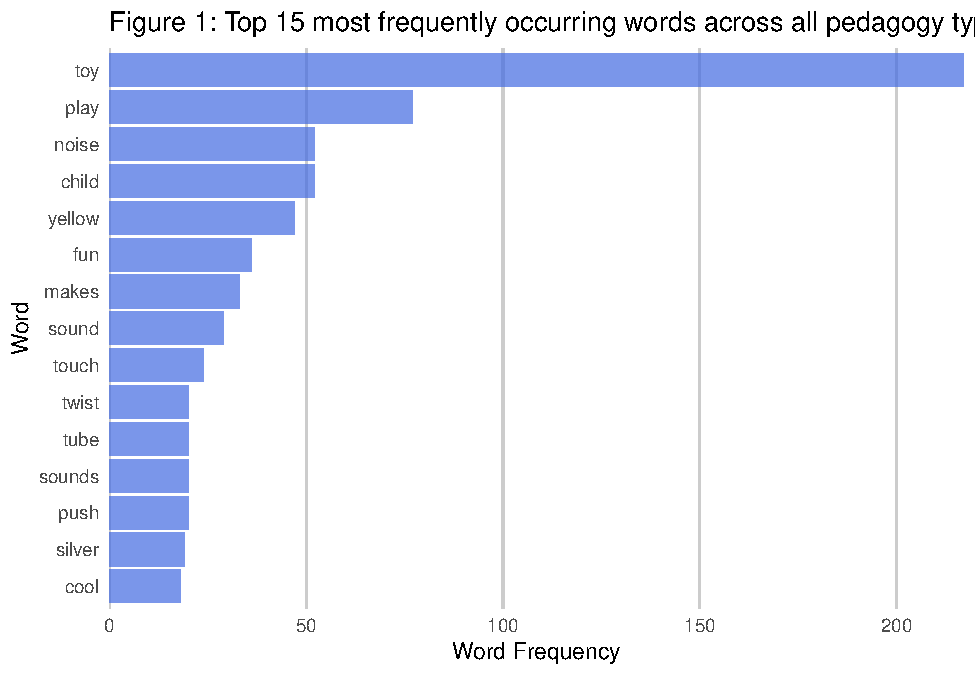
\includegraphics{capstone640_files/figure-latex/initial plots-1.pdf}

\hypertarget{figure-2-word-frequency-cloud-across-conditions}{%
\section{Figure 2: Word Frequency Cloud (Across Conditions)}\label{figure-2-word-frequency-cloud-across-conditions}}

\begin{Shaded}
\begin{Highlighting}[]
\CommentTok{\# visualing: word cloud}
\FunctionTok{library}\NormalTok{(wordcloud)}

\NormalTok{tokens }\OtherTok{=}\NormalTok{ textdata }\SpecialCharTok{\%\textgreater{}\%}
  \FunctionTok{unnest\_tokens}\NormalTok{(word, text) }\SpecialCharTok{\%\textgreater{}\%}
  \FunctionTok{anti\_join}\NormalTok{(stop\_words)}

\CommentTok{\# top words}
\NormalTok{word\_count }\OtherTok{=}\NormalTok{ tokens}\SpecialCharTok{\%\textgreater{}\%}
  \FunctionTok{group\_by}\NormalTok{(word)}\SpecialCharTok{\%\textgreater{}\%}
  \FunctionTok{summarise}\NormalTok{(}\AttributeTok{count =} \FunctionTok{n}\NormalTok{())}\SpecialCharTok{\%\textgreater{}\%}
  \FunctionTok{arrange}\NormalTok{(}\FunctionTok{desc}\NormalTok{(count))}\SpecialCharTok{\%\textgreater{}\%}
  \FunctionTok{slice}\NormalTok{(}\DecValTok{1}\SpecialCharTok{:}\DecValTok{10}\NormalTok{)}


\CommentTok{\# word cloud{-}{-}zoom in}
\NormalTok{cloud }\OtherTok{\textless{}{-}}\NormalTok{ tokens }\SpecialCharTok{\%\textgreater{}\%}
  \FunctionTok{group\_by}\NormalTok{(source, word) }\SpecialCharTok{\%\textgreater{}\%}
  \FunctionTok{summarise}\NormalTok{(}\AttributeTok{count =} \FunctionTok{n}\NormalTok{())}\SpecialCharTok{\%\textgreater{}\%}
  \FunctionTok{arrange}\NormalTok{(}\FunctionTok{desc}\NormalTok{(count))}\SpecialCharTok{\%\textgreater{}\%}
  \FunctionTok{slice}\NormalTok{(}\DecValTok{1}\SpecialCharTok{:}\DecValTok{10}\NormalTok{)}
  

\FunctionTok{wordcloud}\NormalTok{(tokens}\SpecialCharTok{$}\NormalTok{word, }\AttributeTok{max.words =} \DecValTok{75}\NormalTok{, }\AttributeTok{colors=}\FunctionTok{brewer.pal}\NormalTok{(}\DecValTok{6}\NormalTok{, }\StringTok{"Dark2"}\NormalTok{))}
\end{Highlighting}
\end{Shaded}

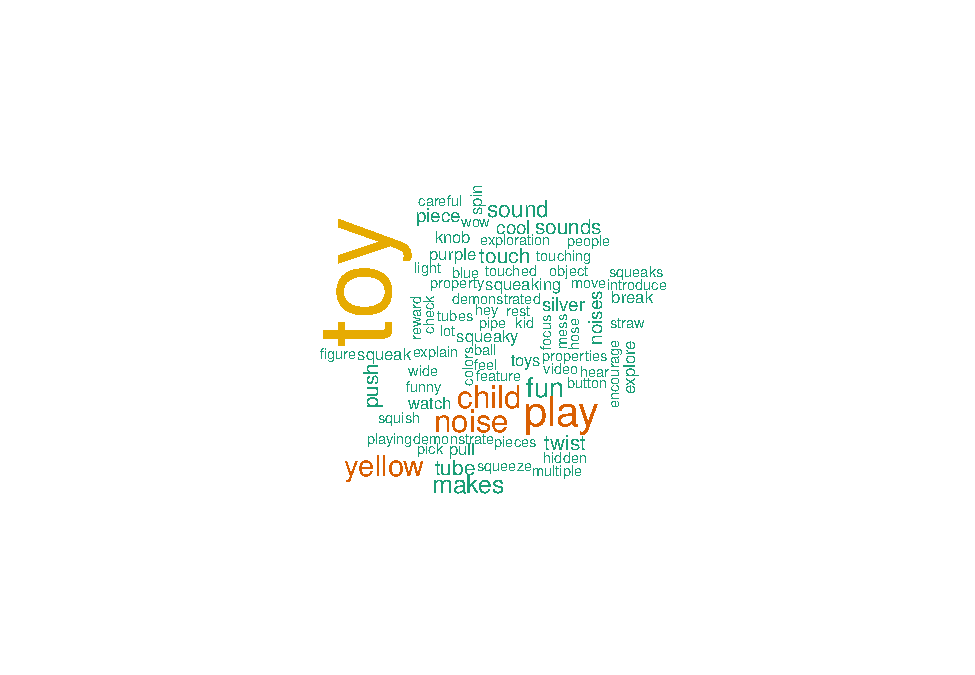
\includegraphics{capstone640_files/figure-latex/word cloud-1.pdf}

\begin{Shaded}
\begin{Highlighting}[]
\NormalTok{tidy\_words }\SpecialCharTok{\%\textgreater{}\%} 
  \FunctionTok{group\_by}\NormalTok{(condition) }\SpecialCharTok{\%\textgreater{}\%}
  \FunctionTok{anti\_join}\NormalTok{(stop\_words) }\SpecialCharTok{\%\textgreater{}\%} 
  \FunctionTok{count}\NormalTok{(word, }\AttributeTok{sort =} \ConstantTok{TRUE}\NormalTok{) }\SpecialCharTok{\%\textgreater{}\%} 
  \FunctionTok{mutate}\NormalTok{(}\AttributeTok{word =} \FunctionTok{reorder}\NormalTok{(word, n)) }\SpecialCharTok{\%\textgreater{}\%} \CommentTok{\# make y{-}axis ordered by n}
  \FunctionTok{slice}\NormalTok{(}\DecValTok{1}\SpecialCharTok{:}\DecValTok{15}\NormalTok{) }\SpecialCharTok{\%\textgreater{}\%} \CommentTok{\# select only the first 15 rows}
  \FunctionTok{ggplot}\NormalTok{(}\FunctionTok{aes}\NormalTok{(n, word, }\AttributeTok{fill =}\NormalTok{ condition)) }\SpecialCharTok{+}
  \FunctionTok{geom\_col}\NormalTok{(}\AttributeTok{alpha =}\NormalTok{ .}\DecValTok{7}\NormalTok{) }\SpecialCharTok{+}
  \FunctionTok{facet\_wrap}\NormalTok{(}\SpecialCharTok{\textasciitilde{}}\NormalTok{condition) }\SpecialCharTok{+}
  \FunctionTok{scale\_x\_continuous}\NormalTok{(}\AttributeTok{expand =} \FunctionTok{c}\NormalTok{(}\DecValTok{0}\NormalTok{,}\DecValTok{0}\NormalTok{)) }\SpecialCharTok{+}
  \FunctionTok{theme\_minimal}\NormalTok{() }\SpecialCharTok{+}
  \FunctionTok{theme}\NormalTok{(}
    \AttributeTok{panel.grid.major.y =} \FunctionTok{element\_blank}\NormalTok{(),}
    \AttributeTok{panel.grid.minor.x =} \FunctionTok{element\_blank}\NormalTok{(),}
    \AttributeTok{panel.grid.major.x =} \FunctionTok{element\_line}\NormalTok{(}\AttributeTok{color =} \StringTok{"gray80"}\NormalTok{)}
\NormalTok{  ) }\SpecialCharTok{+}
  \FunctionTok{labs}\NormalTok{(}
    \AttributeTok{x =} \StringTok{"Word Frequency"}\NormalTok{,}
    \AttributeTok{y =} \StringTok{"Word"}\NormalTok{,}
    \AttributeTok{title =} \StringTok{"Figure 3: Top 15 most frequently occurring words by condition"}\NormalTok{,}
\NormalTok{  )}
\end{Highlighting}
\end{Shaded}

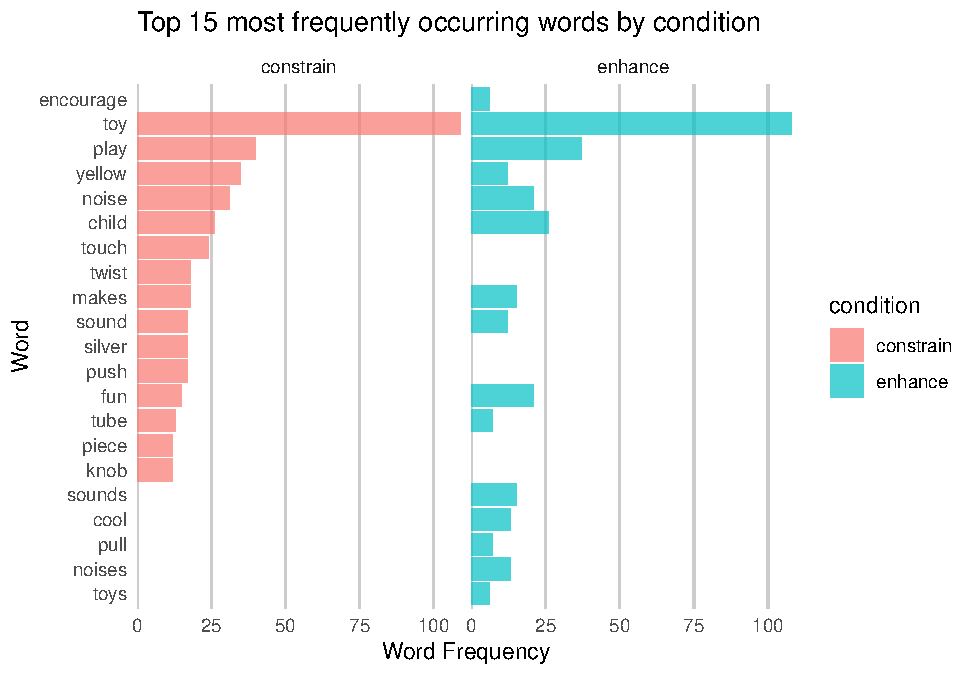
\includegraphics{capstone640_files/figure-latex/unnamed-chunk-1-1.pdf}
In Figure 3, we see the top 15 words used in the enhance and constrain
conditions. In the `enahnce' condition, there was greater use of words like ``sounds,'' ``cool,'' ``pull,'' ``noises,'' and ``toys.'' In the `constrain' condition, there was greater use of ``touch,'' ``silver,'' ``push,'' and ``knob.''

\hypertarget{description-of-sentiment-analysis}{%
\subsubsection{Description of sentiment analysis}\label{description-of-sentiment-analysis}}

After trying for many hours to use the `transformers' package from `huggingface' via
a virtual python environment without success, we decided to utilize sentiment
analysis program from ``bing'' to perform analyses for Model 1. We also utilized three
other programs (``afinn,'' ``loughran,'' and ``nrc''), and a summary of their positive and
negative assessments by condition is included in Table 1 at the end of this
document.Results indicate that pedagogy did not differ significantly in sentiment based upon the condition participants were in.

\begin{Shaded}
\begin{Highlighting}[]
\NormalTok{sentimentdata }\OtherTok{\textless{}{-}} \FunctionTok{import}\NormalTok{(}\FunctionTok{here}\NormalTok{(}\StringTok{"data"}\NormalTok{, }\StringTok{"sentiment\_an.xlsx"}\NormalTok{))}
\NormalTok{sentiment }\OtherTok{\textless{}{-}} \FunctionTok{import}\NormalTok{(}\FunctionTok{here}\NormalTok{(}\StringTok{"data"}\NormalTok{, }\StringTok{"sentiment.xlsx"}\NormalTok{))}

\NormalTok{sentiment\_by\_condition }\OtherTok{\textless{}{-}}\NormalTok{ sentimentdata }\SpecialCharTok{\%\textgreater{}\%}
  \FunctionTok{group\_by}\NormalTok{(condition, analysis) }\SpecialCharTok{\%\textgreater{}\%}
  \FunctionTok{count}\NormalTok{(sentiment)}

\CommentTok{\# table of sentiment for four groups ("bing", "nrc", "afinn", "loughran")}
\NormalTok{sentimenttable }\OtherTok{\textless{}{-}} \FunctionTok{import}\NormalTok{(}\FunctionTok{here}\NormalTok{(}\StringTok{"data"}\NormalTok{, }\StringTok{"sentiment\_table.xlsx"}\NormalTok{))}
\NormalTok{table }\OtherTok{\textless{}{-}}\NormalTok{ sentimenttable[}\DecValTok{1}\SpecialCharTok{:}\DecValTok{2}\NormalTok{, }\DecValTok{2}\SpecialCharTok{:}\DecValTok{11}\NormalTok{]}

\FunctionTok{options}\NormalTok{(}\AttributeTok{kableExtra.auto\_format =} \ConstantTok{FALSE}\NormalTok{)}
\FunctionTok{library}\NormalTok{(kableExtra)}


\NormalTok{table }\SpecialCharTok{\%\textgreater{}\%} 
  \FunctionTok{kbl}\NormalTok{(}\AttributeTok{caption =} \StringTok{"Sentiment by analysis tool"}\NormalTok{) }\SpecialCharTok{\%\textgreater{}\%}
  \FunctionTok{kable\_classic}\NormalTok{(}\AttributeTok{html\_font =} \StringTok{"Cambria"}\NormalTok{) }\SpecialCharTok{\%\textgreater{}\%}
  \FunctionTok{column\_spec}\NormalTok{(}\AttributeTok{column =} \DecValTok{1}\SpecialCharTok{:}\DecValTok{10}\NormalTok{, }\AttributeTok{width =} \StringTok{"0.57in"}\NormalTok{) }\SpecialCharTok{\%\textgreater{}\%}
  \FunctionTok{footnote}\NormalTok{(}\AttributeTok{general\_title =} \StringTok{"Note."}\NormalTok{, }\AttributeTok{footnote\_as\_chunk=}\ConstantTok{TRUE}\NormalTok{, }\AttributeTok{threeparttable=}\ConstantTok{TRUE}\NormalTok{, }\AttributeTok{general =} \StringTok{"Positive (Pos) and Negative (Neg) sentiment analysis by individual words using 4 analysis tools: bing, nrc, loughran, and afinn. Results demonstrate that Total Positive \& Negative sentiment was roughly equal by condition (enhance or constrain). However, positive sentiment was slightly higher for the enhance condition and negative sentiment was slight higher for the constrain condition, which is the expected result."}\NormalTok{) }
\end{Highlighting}
\end{Shaded}

\begin{table}

\caption{(\#tab:sent anal)Sentiment by analysis tool}
\centering
\begin{threeparttable}
\begin{tabular}[t]{>{\raggedleft\arraybackslash}p{0.57in}|>{\raggedleft\arraybackslash}p{0.57in}|>{\raggedleft\arraybackslash}p{0.57in}|>{\raggedleft\arraybackslash}p{0.57in}|>{\raggedleft\arraybackslash}p{0.57in}|>{\raggedleft\arraybackslash}p{0.57in}|>{\raggedleft\arraybackslash}p{0.57in}|>{\raggedleft\arraybackslash}p{0.57in}|>{\raggedleft\arraybackslash}p{0.57in}|>{\raggedleft\arraybackslash}p{0.57in}}
\hline
Pos bing & Neg bing & Pos nrc & Neg nrc & Pos loughran & Neg loughran & Pos afinn & Neg afinn & Total Positive & Total Negative\\
\hline
64 & 66 & 277 & 73 & 18 & 73 & 61 & 10 & 420 & 222\\
\hline
41 & 116 & 274 & 94 & 40 & 28 & 54 & 26 & 409 & 264\\
\hline
\end{tabular}
\begin{tablenotes}[para]
\item \textit{Note.} 
\item Positive (Pos) and Negative (Neg) sentiment analysis by individual words using 4 analysis tools: bing, nrc, loughran, and afinn. Results demonstrate that Total Positive \& Negative sentiment was roughly equal by condition (enhance or constrain). However, positive sentiment was slightly higher for the enhance condition and negative sentiment was slight higher for the constrain condition, which is the expected result.
\end{tablenotes}
\end{threeparttable}
\end{table}

\hypertarget{model-1-predicting-a-categorical-outcome-sentiment-positive-or-negative-using-regularized-logistic-regression}{%
\subsection{Model 1: Predicting a Categorical Outcome (sentiment: positive or negative) using Regularized Logistic Regression}\label{model-1-predicting-a-categorical-outcome-sentiment-positive-or-negative-using-regularized-logistic-regression}}

\begin{Shaded}
\begin{Highlighting}[]
\CommentTok{\# Recipe for the sentiment dataset}

\NormalTok{outcome }\OtherTok{\textless{}{-}} \FunctionTok{c}\NormalTok{(}\StringTok{\textquotesingle{}sentiment\textquotesingle{}}\NormalTok{)}

\NormalTok{ID }\OtherTok{\textless{}{-}} \FunctionTok{c}\NormalTok{(}\StringTok{\textquotesingle{}id\textquotesingle{}}\NormalTok{)}

\NormalTok{categorical }\OtherTok{\textless{}{-}} \FunctionTok{c}\NormalTok{(}\StringTok{\textquotesingle{}condition\textquotesingle{}}\NormalTok{, }\StringTok{\textquotesingle{}source\textquotesingle{}}\NormalTok{, }\StringTok{\textquotesingle{}function\textquotesingle{}}\NormalTok{)}

\NormalTok{ blueprint }\OtherTok{\textless{}{-}} \FunctionTok{recipe}\NormalTok{(}\AttributeTok{x  =}\NormalTok{ sentiment,}
                    \AttributeTok{vars  =} \FunctionTok{c}\NormalTok{(categorical, outcome, ID),}
                    \AttributeTok{roles =} \FunctionTok{c}\NormalTok{(}\FunctionTok{rep}\NormalTok{(}\StringTok{\textquotesingle{}predictor\textquotesingle{}}\NormalTok{,}\DecValTok{3}\NormalTok{), }\StringTok{\textquotesingle{}outcome\textquotesingle{}}\NormalTok{, }\StringTok{\textquotesingle{}ID\textquotesingle{}}\NormalTok{)) }\SpecialCharTok{\%\textgreater{}\%}
  \FunctionTok{step\_zv}\NormalTok{(}\FunctionTok{all\_of}\NormalTok{(categorical)) }


\CommentTok{\# splitting data into training and testing}
\CommentTok{\# Let the training data have the 80\% of cases and the test data have the 20\% of the cases.}

\FunctionTok{set.seed}\NormalTok{(}\DecValTok{11102021}\NormalTok{)  }\CommentTok{\# for reproducibility}
  
\NormalTok{sen      }\OtherTok{\textless{}{-}} \FunctionTok{sample}\NormalTok{(}\DecValTok{1}\SpecialCharTok{:}\FunctionTok{nrow}\NormalTok{(sentiment), }\FunctionTok{round}\NormalTok{(}\FunctionTok{nrow}\NormalTok{(sentiment) }\SpecialCharTok{*} \FloatTok{0.8}\NormalTok{))}
\NormalTok{sen\_train  }\OtherTok{\textless{}{-}}\NormalTok{ sentiment[sen, ]}
\NormalTok{sen\_test  }\OtherTok{\textless{}{-}}\NormalTok{ sentiment[}\SpecialCharTok{{-}}\NormalTok{sen, ]}

\CommentTok{\# 10{-}fold cross{-}validation without regularization}

\FunctionTok{set.seed}\NormalTok{(}\DecValTok{11152021}\NormalTok{) }\CommentTok{\# for reproducibility}

\NormalTok{sen\_tr }\OtherTok{=}\NormalTok{ sen\_train[}\FunctionTok{sample}\NormalTok{(}\FunctionTok{nrow}\NormalTok{(sen\_train)),]}

  \CommentTok{\# Creating 10 folds with equal size}

\NormalTok{folds }\OtherTok{=} \FunctionTok{cut}\NormalTok{(}\FunctionTok{seq}\NormalTok{(}\DecValTok{1}\NormalTok{,}\FunctionTok{nrow}\NormalTok{(sen\_tr)),}\AttributeTok{breaks=}\DecValTok{10}\NormalTok{,}\AttributeTok{labels=}\ConstantTok{FALSE}\NormalTok{)}
  
  \CommentTok{\# Creating the list for each fold }
\NormalTok{sen.indices }\OtherTok{\textless{}{-}} \FunctionTok{vector}\NormalTok{(}\StringTok{\textquotesingle{}list\textquotesingle{}}\NormalTok{,}\DecValTok{10}\NormalTok{)}

      \ControlFlowTok{for}\NormalTok{(i }\ControlFlowTok{in} \DecValTok{1}\SpecialCharTok{:}\DecValTok{10}\NormalTok{)\{}
\NormalTok{        sen.indices[[i]] }\OtherTok{\textless{}{-}} \FunctionTok{which}\NormalTok{(folds}\SpecialCharTok{!=}\NormalTok{i)}
\NormalTok{      \}}
    

\NormalTok{ cv }\OtherTok{\textless{}{-}} \FunctionTok{trainControl}\NormalTok{(}\AttributeTok{method    =} \StringTok{"cv"}\NormalTok{,}
                   \AttributeTok{index           =}\NormalTok{ sen.indices,}
                   \AttributeTok{classProbs      =} \ConstantTok{TRUE}\NormalTok{,}
                   \AttributeTok{summaryFunction =}\NormalTok{ mnLogLoss)}
    
      
\CommentTok{\# Train the model}
\NormalTok{ caret\_mod }\OtherTok{\textless{}{-}}\NormalTok{ caret}\SpecialCharTok{::}\FunctionTok{train}\NormalTok{(blueprint, }
                          \AttributeTok{data      =}\NormalTok{ sen\_tr, }
                          \AttributeTok{method    =} \StringTok{"glm"}\NormalTok{,}
                          \AttributeTok{family    =} \StringTok{\textquotesingle{}binomial\textquotesingle{}}\NormalTok{,}
                          \AttributeTok{metric    =} \StringTok{\textquotesingle{}logLoss\textquotesingle{}}\NormalTok{,}
                          \AttributeTok{trControl =}\NormalTok{ cv)}
 
\CommentTok{\# caret\_mod}
 
 \CommentTok{\# Evaluate the model on the test data}

\CommentTok{\# Predict the probabilities for the observations in the test dataset}
 
\NormalTok{ predicted\_test }\OtherTok{\textless{}{-}} \FunctionTok{predict}\NormalTok{(caret\_mod, sen\_test, }\AttributeTok{type=}\StringTok{\textquotesingle{}prob\textquotesingle{}}\NormalTok{)}

\CommentTok{\# head(predicted\_test)}


\CommentTok{\# Evaluate the model on the test dataset}
\NormalTok{predicted\_te }\OtherTok{\textless{}{-}} \FunctionTok{predict}\NormalTok{(caret\_mod, sen\_test)}

\NormalTok{predicted\_te }\OtherTok{\textless{}{-}} \FunctionTok{as.numeric}\NormalTok{(predicted\_te)}
\NormalTok{sen\_test\_numeric }\OtherTok{\textless{}{-}}\NormalTok{ sen\_test}\SpecialCharTok{$}\NormalTok{sentiment\_numeric}


\NormalTok{predicted\_eval }\OtherTok{\textless{}{-}} \FunctionTok{data.frame}\NormalTok{(predicted\_te, sen\_test\_numeric)}
\NormalTok{predicted\_eval }\OtherTok{\textless{}{-}}\NormalTok{ predicted\_eval[}\FunctionTok{complete.cases}\NormalTok{(predicted\_eval), ]}


\NormalTok{rsq\_te }\OtherTok{\textless{}{-}} \FunctionTok{cor}\NormalTok{(predicted\_eval}\SpecialCharTok{$}\NormalTok{predicted\_te,predicted\_eval}\SpecialCharTok{$}\NormalTok{sen\_test\_numeric)}\SpecialCharTok{\^{}}\DecValTok{2}
\CommentTok{\# rsq\_te}

\NormalTok{mae\_te }\OtherTok{\textless{}{-}} \FunctionTok{mean}\NormalTok{(}\FunctionTok{abs}\NormalTok{(predicted\_eval}\SpecialCharTok{$}\NormalTok{sen\_test\_numeric }\SpecialCharTok{{-}}\NormalTok{ predicted\_eval}\SpecialCharTok{$}\NormalTok{predicted\_te))}
\CommentTok{\# mae\_te}

\NormalTok{rmse\_te }\OtherTok{\textless{}{-}} \FunctionTok{sqrt}\NormalTok{(}\FunctionTok{mean}\NormalTok{((predicted\_eval}\SpecialCharTok{$}\NormalTok{sen\_test\_numeric }\SpecialCharTok{{-}}\NormalTok{ predicted\_eval}\SpecialCharTok{$}\NormalTok{predicted\_te)}\SpecialCharTok{\^{}}\DecValTok{2}\NormalTok{))}
\CommentTok{\# rmse\_te}
\end{Highlighting}
\end{Shaded}

\hypertarget{results-model-1}{%
\section{Results Model 1}\label{results-model-1}}

The first model is a regularized logistic regression predicting sentiment type
(positive or negative) from a participant's condition (enhance or constrain), source
(qualtrics survey or pre-existing study pedagogy) and function (`squeaker' or
'light). Model 1 results indicate that the model may not be capturing the proper
predictors for sentiment (or our previous sentiment analysis--utilizing bing, might
not accurately be representing the sentiment in our sample). It is also possible
that there is no relation between sentiment and condition, source, or function. The
R-squared value indicates the the model is predicting only a fraction of the
proportion of variance (0.026). Similarly, root mean squared error (0.78) and mean
absolute error (0.61) also indicate that the model's predictions are farther away
from the actual values.

\hypertarget{model-2-k-nearest-neighbors-to-predict-rank-ordered-exploration-promotion-from-pedagogy-text-sample}{%
\subsubsection{Model 2: K-nearest neighbors to predict rank ordered exploration-promotion from pedagogy text sample}\label{model-2-k-nearest-neighbors-to-predict-rank-ordered-exploration-promotion-from-pedagogy-text-sample}}

\begin{Shaded}
\begin{Highlighting}[]
\CommentTok{\# import data}
\CommentTok{\# textdummy \textless{}{-} import(here("data", "text\_data\_dummy.xlsx"))}
\NormalTok{ textdummy }\OtherTok{\textless{}{-}}\FunctionTok{import}\NormalTok{(}\FunctionTok{here}\NormalTok{(}\StringTok{"data"}\NormalTok{, }\StringTok{"text\_dummy.xlsx"}\NormalTok{))}

\CommentTok{\# train and test split}

\FunctionTok{set.seed}\NormalTok{(}\DecValTok{10152022}\NormalTok{) }\CommentTok{\# for reproducibility}

\NormalTok{loc }\OtherTok{\textless{}{-}} \FunctionTok{sample}\NormalTok{(}\DecValTok{1}\SpecialCharTok{:}\FunctionTok{nrow}\NormalTok{(textdummy), }\FunctionTok{round}\NormalTok{(}\FunctionTok{nrow}\NormalTok{(textdummy) }\SpecialCharTok{*} \FloatTok{0.9}\NormalTok{))}
\NormalTok{rank\_tr }\OtherTok{\textless{}{-}}\NormalTok{ textdummy[loc, ]}
\NormalTok{rank\_te }\OtherTok{\textless{}{-}}\NormalTok{ textdummy[}\SpecialCharTok{{-}}\NormalTok{loc, ]}


\CommentTok{\# create row indices for 10{-}folds}

  \CommentTok{\#randomly shuffle training data}
\NormalTok{rank\_tr }\OtherTok{=}\NormalTok{ rank\_tr[}\FunctionTok{sample}\NormalTok{(}\FunctionTok{nrow}\NormalTok{(rank\_tr)),]}

    \CommentTok{\# Create 10 folds with equal size}

\NormalTok{      folds }\OtherTok{=} \FunctionTok{cut}\NormalTok{(}\FunctionTok{seq}\NormalTok{(}\DecValTok{1}\NormalTok{,}\FunctionTok{nrow}\NormalTok{(rank\_tr)),}\AttributeTok{breaks=}\DecValTok{10}\NormalTok{,}\AttributeTok{labels=}\ConstantTok{FALSE}\NormalTok{)}
  
    \CommentTok{\# Create the list for each fold }
      
\NormalTok{      my.indices }\OtherTok{\textless{}{-}} \FunctionTok{vector}\NormalTok{(}\StringTok{\textquotesingle{}list\textquotesingle{}}\NormalTok{,}\DecValTok{10}\NormalTok{)}
      \ControlFlowTok{for}\NormalTok{(i }\ControlFlowTok{in} \DecValTok{1}\SpecialCharTok{:}\DecValTok{10}\NormalTok{)\{}
\NormalTok{        my.indices[[i]] }\OtherTok{\textless{}{-}} \FunctionTok{which}\NormalTok{(folds}\SpecialCharTok{!=}\NormalTok{i)}
\NormalTok{      \}}

\CommentTok{\# Cross{-}validation settings}
      
\NormalTok{  cv }\OtherTok{\textless{}{-}} \FunctionTok{trainControl}\NormalTok{(}\AttributeTok{method =} \StringTok{"cv"}\NormalTok{,}
                     \AttributeTok{index  =}\NormalTok{ my.indices)}
  
\FunctionTok{require}\NormalTok{(caret)}
\FunctionTok{require}\NormalTok{(kknn)}

\FunctionTok{getModelInfo}\NormalTok{()}\SpecialCharTok{$}\NormalTok{kknn}\SpecialCharTok{$}\NormalTok{parameters}
\end{Highlighting}
\end{Shaded}

\begin{verbatim}
##   parameter     class           label
## 1      kmax   numeric Max. #Neighbors
## 2  distance   numeric        Distance
## 3    kernel character          Kernel
\end{verbatim}

\begin{Shaded}
\begin{Highlighting}[]
\CommentTok{\# Hyperparameter Tuning Grid}
  
\NormalTok{  grid }\OtherTok{\textless{}{-}} \FunctionTok{expand.grid}\NormalTok{(}\AttributeTok{kmax    =} \DecValTok{3}\SpecialCharTok{:}\DecValTok{25}\NormalTok{,}
                     \AttributeTok{distance =} \FunctionTok{c}\NormalTok{(}\DecValTok{1}\NormalTok{,}\DecValTok{2}\NormalTok{,}\DecValTok{3}\NormalTok{),}
                     \AttributeTok{kernel   =} \FunctionTok{c}\NormalTok{(}\StringTok{\textquotesingle{}epanechnikov\textquotesingle{}}\NormalTok{,}\StringTok{\textquotesingle{}rectangular\textquotesingle{}}\NormalTok{))}
 \CommentTok{\# grid}
  
  
\FunctionTok{require}\NormalTok{(doParallel)}

\NormalTok{ncores }\OtherTok{\textless{}{-}} \DecValTok{8}    

\NormalTok{cl }\OtherTok{\textless{}{-}} \FunctionTok{makePSOCKcluster}\NormalTok{(ncores)}

\FunctionTok{registerDoParallel}\NormalTok{(cl)}


\CommentTok{\# Train the model}

\NormalTok{textdummy}\SpecialCharTok{$}\NormalTok{source }\OtherTok{\textless{}{-}} \FunctionTok{as.vector}\NormalTok{(textdummy}\SpecialCharTok{$}\NormalTok{source)}
\NormalTok{textdummy}\SpecialCharTok{$}\NormalTok{rank }\OtherTok{\textless{}{-}} \FunctionTok{as.vector}\NormalTok{(textdummy}\SpecialCharTok{$}\NormalTok{rank)}
\NormalTok{textdummy}\SpecialCharTok{$}\NormalTok{condition }\OtherTok{\textless{}{-}} \FunctionTok{as.vector}\NormalTok{(textdummy}\SpecialCharTok{$}\NormalTok{condition)}
\NormalTok{textdummy}\SpecialCharTok{$}\NormalTok{funct }\OtherTok{\textless{}{-}} \FunctionTok{as.vector}\NormalTok{(textdummy}\SpecialCharTok{$}\NormalTok{funct)}
\NormalTok{textdummy}\SpecialCharTok{$}\NormalTok{id }\OtherTok{\textless{}{-}} \FunctionTok{as.vector}\NormalTok{(textdummy}\SpecialCharTok{$}\NormalTok{id)}

\NormalTok{outcome }\OtherTok{\textless{}{-}} \FunctionTok{c}\NormalTok{(}\StringTok{\textquotesingle{}rank\textquotesingle{}}\NormalTok{)}

\NormalTok{ID }\OtherTok{\textless{}{-}} \FunctionTok{c}\NormalTok{(}\StringTok{\textquotesingle{}id\textquotesingle{}}\NormalTok{)}

\NormalTok{categorical }\OtherTok{\textless{}{-}} \FunctionTok{c}\NormalTok{(}\StringTok{\textquotesingle{}condition\textquotesingle{}}\NormalTok{, }\StringTok{\textquotesingle{}source\textquotesingle{}}\NormalTok{, }\StringTok{\textquotesingle{}funct\textquotesingle{}}\NormalTok{)}

\NormalTok{blueprint\_textdummy }\OtherTok{\textless{}{-}} \FunctionTok{recipe}\NormalTok{(}\AttributeTok{x  =}\NormalTok{ textdummy,}
                    \AttributeTok{vars  =} \FunctionTok{c}\NormalTok{(categorical, outcome, ID),}
                    \AttributeTok{roles =} \FunctionTok{c}\NormalTok{(}\FunctionTok{rep}\NormalTok{(}\StringTok{\textquotesingle{}predictor\textquotesingle{}}\NormalTok{,}\DecValTok{3}\NormalTok{), }\StringTok{\textquotesingle{}outcome\textquotesingle{}}\NormalTok{, }\StringTok{\textquotesingle{}ID\textquotesingle{}}\NormalTok{)) }


\NormalTok{  caret\_knn }\OtherTok{\textless{}{-}}\NormalTok{ caret}\SpecialCharTok{::}\FunctionTok{train}\NormalTok{(blueprint\_textdummy, }
                                        \AttributeTok{data      =}\NormalTok{ rank\_tr,}
                                        \AttributeTok{method    =} \StringTok{"kknn"}\NormalTok{,}
                                        \AttributeTok{trControl =}\NormalTok{ cv,}
                                        \AttributeTok{tuneGrid  =}\NormalTok{ grid)}
  
  \FunctionTok{plot}\NormalTok{(caret\_knn)}
\end{Highlighting}
\end{Shaded}

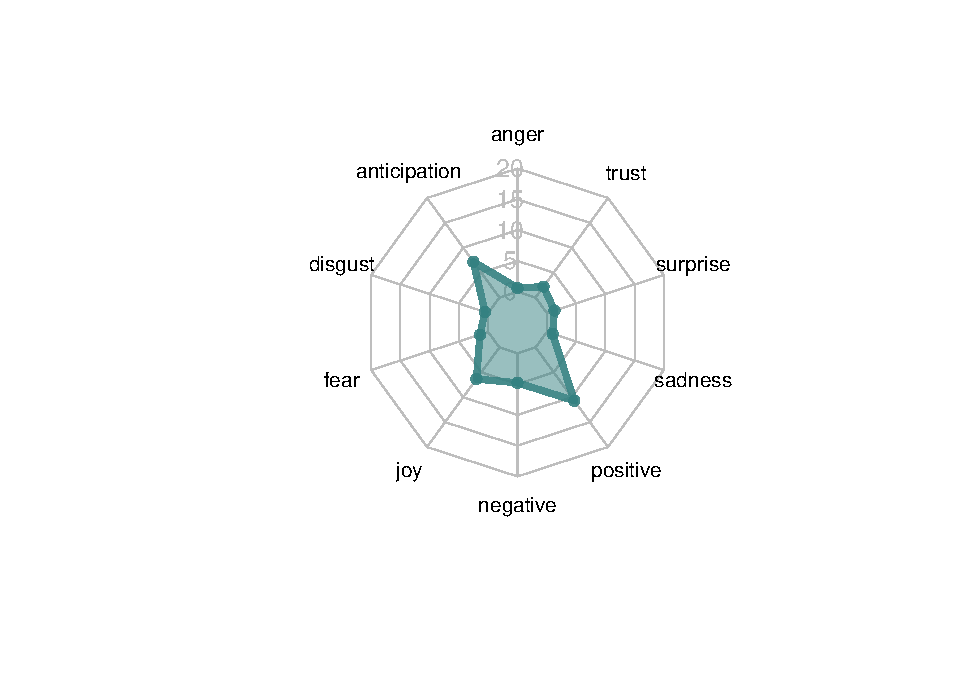
\includegraphics{capstone640_files/figure-latex/unnamed-chunk-4-1.pdf}

\begin{Shaded}
\begin{Highlighting}[]
\NormalTok{  caret\_knn}\SpecialCharTok{$}\NormalTok{bestTune}
\end{Highlighting}
\end{Shaded}

\begin{verbatim}
##     kmax distance      kernel
## 136   25        2 rectangular
\end{verbatim}

\begin{Shaded}
\begin{Highlighting}[]
\CommentTok{\# checking performance of knn algorithm on test dataset}
\NormalTok{predicted\_te }\OtherTok{\textless{}{-}} \FunctionTok{predict}\NormalTok{(caret\_knn}\SpecialCharTok{$}\NormalTok{finalModel, }\AttributeTok{newdata =}\NormalTok{ rank\_te)}

\CommentTok{\# r{-}square}
\FunctionTok{cor}\NormalTok{(rank\_te}\SpecialCharTok{$}\NormalTok{rank, predicted\_te)}\SpecialCharTok{\^{}}\DecValTok{2}
\end{Highlighting}
\end{Shaded}

\begin{verbatim}
## [1] 0.6127713
\end{verbatim}

\begin{Shaded}
\begin{Highlighting}[]
\CommentTok{\# rmse}
\FunctionTok{sqrt}\NormalTok{(}\FunctionTok{mean}\NormalTok{((rank\_te}\SpecialCharTok{$}\NormalTok{rank }\SpecialCharTok{{-}}\NormalTok{ predicted\_te)}\SpecialCharTok{*}\DecValTok{2}\NormalTok{))}
\end{Highlighting}
\end{Shaded}

\begin{verbatim}
## [1] 0.85
\end{verbatim}

\begin{Shaded}
\begin{Highlighting}[]
\CommentTok{\# mae}
\FunctionTok{mean}\NormalTok{(}\FunctionTok{abs}\NormalTok{(rank\_te}\SpecialCharTok{$}\NormalTok{rank }\SpecialCharTok{{-}}\NormalTok{predicted\_te))}
\end{Highlighting}
\end{Shaded}

\begin{verbatim}
## [1] 0.94125
\end{verbatim}

\hypertarget{results-model-2}{%
\section{Results Model 2}\label{results-model-2}}

In Model 2, we trained a k nearest neighbor model with a rank outcome (7-point
likert scale representing the likelihood a given pedagogical text will illicit a
certain behavior). We utilized the same predictors as in Model 1 (condition, source,
function). The resultant R-square value of 0.61 indicates that 61\% of the variance
in the outcome is explained by our model. However, we also obtained a root mean
squared error of 0.85 and a mean absolute error value of 0.94, indicating that our
model had a fair degree of error in its predictions. The results suggest that our
model is an okay fit, but we should likely investigate other predictors for best
fit.

\hypertarget{model-3-logistic-regression-predicting-whether-the-target-function-was-discovered}{%
\subsubsection{Model 3: Logistic regression predicting whether the target function was discovered}\label{model-3-logistic-regression-predicting-whether-the-target-function-was-discovered}}

\begin{Shaded}
\begin{Highlighting}[]
\CommentTok{\# omsi \textless{}{-} import(here("data", "omsidata.xlsx"))}
\NormalTok{omsi }\OtherTok{\textless{}{-}} \FunctionTok{import}\NormalTok{(}\FunctionTok{here}\NormalTok{(}\StringTok{"data"}\NormalTok{, }\StringTok{"omsi.xlsx"}\NormalTok{))}

\NormalTok{outcome }\OtherTok{\textless{}{-}} \FunctionTok{c}\NormalTok{(}\StringTok{\textquotesingle{}squeaker\_discovered\textquotesingle{}}\NormalTok{)}

\NormalTok{ID }\OtherTok{\textless{}{-}} \FunctionTok{c}\NormalTok{(}\StringTok{\textquotesingle{}participant\textquotesingle{}}\NormalTok{)}

\NormalTok{categorical }\OtherTok{\textless{}{-}} \FunctionTok{c}\NormalTok{(}\StringTok{\textquotesingle{}condition\textquotesingle{}}\NormalTok{, }\StringTok{\textquotesingle{}gender\textquotesingle{}}\NormalTok{, }\StringTok{\textquotesingle{}total\_time\textquotesingle{}}\NormalTok{, }\StringTok{\textquotesingle{}unique\_actions\textquotesingle{}}\NormalTok{, }\StringTok{\textquotesingle{}squeak\_time\textquotesingle{}}\NormalTok{, }\StringTok{\textquotesingle{}target\_functions\textquotesingle{}}\NormalTok{, }\StringTok{\textquotesingle{}total\_functions\textquotesingle{}}\NormalTok{, }\StringTok{\textquotesingle{}age\_months\textquotesingle{}}\NormalTok{)}

\CommentTok{\# old blueprint for data w/ character values:}
\CommentTok{\# blueprint \textless{}{-} recipe(x  = omsi,}
\CommentTok{\#                    vars  = c(categorical, outcome, ID),}
\CommentTok{\#                    roles = c(rep(\textquotesingle{}predictor\textquotesingle{}),\textquotesingle{}outcome\textquotesingle{},\textquotesingle{}ID\textquotesingle{})) \%\textgreater{}\%}
\CommentTok{\#  step\_indicate\_na(all\_of(categorical)) \%\textgreater{}\%}
\CommentTok{\#  step\_zv(all\_of(categorical)) \%\textgreater{}\%}
\CommentTok{\#    step\_num2factor(outcome,}
\CommentTok{\#                  transform = function(x) x + 1,}
\CommentTok{\#                  levels=c(\textquotesingle{}Y\textquotesingle{}, \textquotesingle{}N\textquotesingle{})) \%\textgreater{}\%}
\CommentTok{\#  step\_num2factor(condition, }
\CommentTok{\#                  transform = function(x) x + 1,}
\CommentTok{\#                  levels=c(\textquotesingle{}ped1\textquotesingle{}, \textquotesingle{}baseline\textquotesingle{}, \textquotesingle{}interrupted\textquotesingle{}, \textquotesingle{}naive\textquotesingle{}))}
 
 
\CommentTok{\# omsi blueprint}
\NormalTok{ blueprint }\OtherTok{\textless{}{-}} \FunctionTok{recipe}\NormalTok{(}\AttributeTok{x  =}\NormalTok{ omsi,}
                    \AttributeTok{vars  =} \FunctionTok{colnames}\NormalTok{(omsi),}
                    \AttributeTok{roles =} \FunctionTok{c}\NormalTok{(}\FunctionTok{rep}\NormalTok{(}\StringTok{\textquotesingle{}predictor\textquotesingle{}}\NormalTok{,}\DecValTok{8}\NormalTok{), }\StringTok{\textquotesingle{}outcome\textquotesingle{}}\NormalTok{, }\StringTok{\textquotesingle{}ID\textquotesingle{}}\NormalTok{)) }\SpecialCharTok{\%\textgreater{}\%}
   \FunctionTok{step\_zv}\NormalTok{(}\FunctionTok{all\_numeric}\NormalTok{()) }\SpecialCharTok{\%\textgreater{}\%}
    \FunctionTok{step\_nzv}\NormalTok{(}\FunctionTok{all\_numeric}\NormalTok{()) }\SpecialCharTok{\%\textgreater{}\%}
    \FunctionTok{step\_impute\_mean}\NormalTok{(}\FunctionTok{all\_numeric}\NormalTok{()) }\SpecialCharTok{\%\textgreater{}\%}
    \FunctionTok{step\_normalize}\NormalTok{(}\FunctionTok{all\_numeric\_predictors}\NormalTok{()) }\SpecialCharTok{\%\textgreater{}\%}
    \FunctionTok{step\_corr}\NormalTok{(}\FunctionTok{all\_numeric}\NormalTok{(),}\AttributeTok{threshold=}\FloatTok{0.9}\NormalTok{)}


\CommentTok{\# splitting data into training and testing}
\CommentTok{\# Let the training data have the 80\% of cases and the test data have the 20\% of the cases.}

\FunctionTok{set.seed}\NormalTok{(}\DecValTok{11102021}\NormalTok{)  }\CommentTok{\# for reproducibility}
  
\NormalTok{om     }\OtherTok{\textless{}{-}} \FunctionTok{sample}\NormalTok{(}\DecValTok{1}\SpecialCharTok{:}\FunctionTok{nrow}\NormalTok{(omsi), }\FunctionTok{round}\NormalTok{(}\FunctionTok{nrow}\NormalTok{(omsi) }\SpecialCharTok{*} \FloatTok{0.8}\NormalTok{))}
\NormalTok{omsi\_tr  }\OtherTok{\textless{}{-}}\NormalTok{ omsi[om, ]}
\NormalTok{omsi\_te}\OtherTok{\textless{}{-}}\NormalTok{ omsi[}\SpecialCharTok{{-}}\NormalTok{om, ]}

\CommentTok{\# 10{-}fold cross{-}validation without regularization}

\NormalTok{omsi\_tr }\OtherTok{=}\NormalTok{ omsi\_tr[}\FunctionTok{sample}\NormalTok{(}\FunctionTok{nrow}\NormalTok{(omsi\_tr)),]}

  \CommentTok{\# Creating 10 folds with equal size}

\NormalTok{folds }\OtherTok{=} \FunctionTok{cut}\NormalTok{(}\FunctionTok{seq}\NormalTok{(}\DecValTok{1}\NormalTok{,}\FunctionTok{nrow}\NormalTok{(omsi\_tr)),}\AttributeTok{breaks=}\DecValTok{10}\NormalTok{,}\AttributeTok{labels=}\ConstantTok{FALSE}\NormalTok{)}
  
  \CommentTok{\# Creating the list for each fold }
\NormalTok{sen.indices }\OtherTok{\textless{}{-}} \FunctionTok{vector}\NormalTok{(}\StringTok{\textquotesingle{}list\textquotesingle{}}\NormalTok{,}\DecValTok{10}\NormalTok{)}

      \ControlFlowTok{for}\NormalTok{(i }\ControlFlowTok{in} \DecValTok{1}\SpecialCharTok{:}\DecValTok{10}\NormalTok{)\{}
\NormalTok{        sen.indices[[i]] }\OtherTok{\textless{}{-}} \FunctionTok{which}\NormalTok{(folds}\SpecialCharTok{!=}\NormalTok{i)}
\NormalTok{      \}}
    

\NormalTok{ cv }\OtherTok{\textless{}{-}} \FunctionTok{trainControl}\NormalTok{(}\AttributeTok{method    =} \StringTok{"cv"}\NormalTok{,}
                   \AttributeTok{index           =}\NormalTok{ sen.indices)}
    
\CommentTok{\# Train the model}
\NormalTok{ grid }\OtherTok{\textless{}{-}} \FunctionTok{data.frame}\NormalTok{ (}\AttributeTok{alpha =} \DecValTok{0}\NormalTok{, }\AttributeTok{lambda=} \FunctionTok{seq}\NormalTok{(}\FloatTok{0.01}\NormalTok{, }\DecValTok{3}\NormalTok{, .}\DecValTok{01}\NormalTok{))}
 
\NormalTok{ ridge }\OtherTok{\textless{}{-}}\NormalTok{ caret}\SpecialCharTok{::}\FunctionTok{train}\NormalTok{(blueprint, }
                          \AttributeTok{data      =}\NormalTok{ omsi\_tr, }
                          \AttributeTok{method    =} \StringTok{"glmnet"}\NormalTok{,}
                          \AttributeTok{trControl =}\NormalTok{ cv, }
                          \AttributeTok{tuneGrid =}\NormalTok{ grid)}
 
\CommentTok{\# ridge$results}
\NormalTok{ ridge}\SpecialCharTok{$}\NormalTok{bestTune}
\end{Highlighting}
\end{Shaded}

\begin{verbatim}
##   alpha lambda
## 6     0   0.06
\end{verbatim}

\begin{Shaded}
\begin{Highlighting}[]
 \FunctionTok{plot}\NormalTok{(ridge)}
\end{Highlighting}
\end{Shaded}

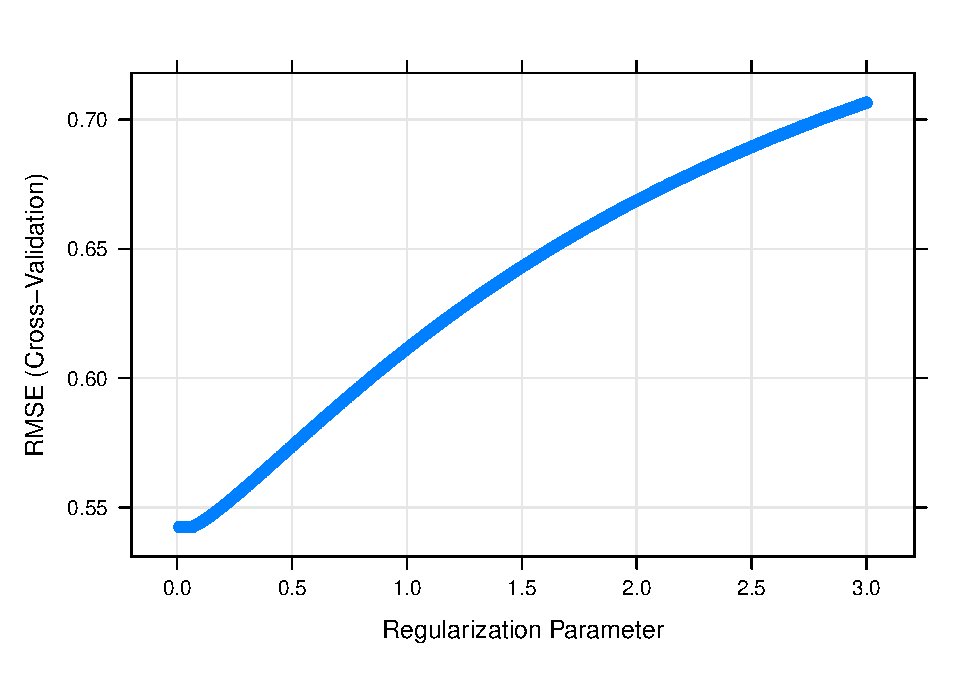
\includegraphics{capstone640_files/figure-latex/unnamed-chunk-5-1.pdf}

\begin{Shaded}
\begin{Highlighting}[]
 \CommentTok{\# Evaluate the model on the test data}

\CommentTok{\# Predict the probabilities for the observations in the test dataset}
 
\NormalTok{ predicted\_te\_ridge }\OtherTok{\textless{}{-}} \FunctionTok{predict}\NormalTok{(ridge, omsi\_te)}

\NormalTok{rsq\_te }\OtherTok{\textless{}{-}} \FunctionTok{cor}\NormalTok{(predicted\_te\_ridge, omsi\_te}\SpecialCharTok{$}\NormalTok{squeaker\_discovered)}\SpecialCharTok{\^{}}\DecValTok{2}  
\CommentTok{\# rsq\_te}

\NormalTok{mae\_te }\OtherTok{\textless{}{-}} \FunctionTok{mean}\NormalTok{(}\FunctionTok{abs}\NormalTok{(omsi\_te}\SpecialCharTok{$}\NormalTok{squeaker\_discovered }\SpecialCharTok{{-}}\NormalTok{ predicted\_te\_ridge))}
\CommentTok{\# mae\_te}

\NormalTok{rmse\_te }\OtherTok{\textless{}{-}} \FunctionTok{sqrt}\NormalTok{(}\FunctionTok{mean}\NormalTok{((omsi\_te}\SpecialCharTok{$}\NormalTok{squeaker\_discovered }\SpecialCharTok{{-}}\NormalTok{predicted\_te\_ridge)}\SpecialCharTok{\^{}}\DecValTok{2}\NormalTok{))}
\CommentTok{\# rmse\_te}



\CommentTok{\# variable importance}
\FunctionTok{require}\NormalTok{(vip)}

\FunctionTok{vip}\NormalTok{(ridge, }\AttributeTok{num\_features =} \DecValTok{10}\NormalTok{, }\AttributeTok{geom =} \StringTok{"point"}\NormalTok{) }\SpecialCharTok{+} 
  \FunctionTok{theme\_bw}\NormalTok{()}
\end{Highlighting}
\end{Shaded}

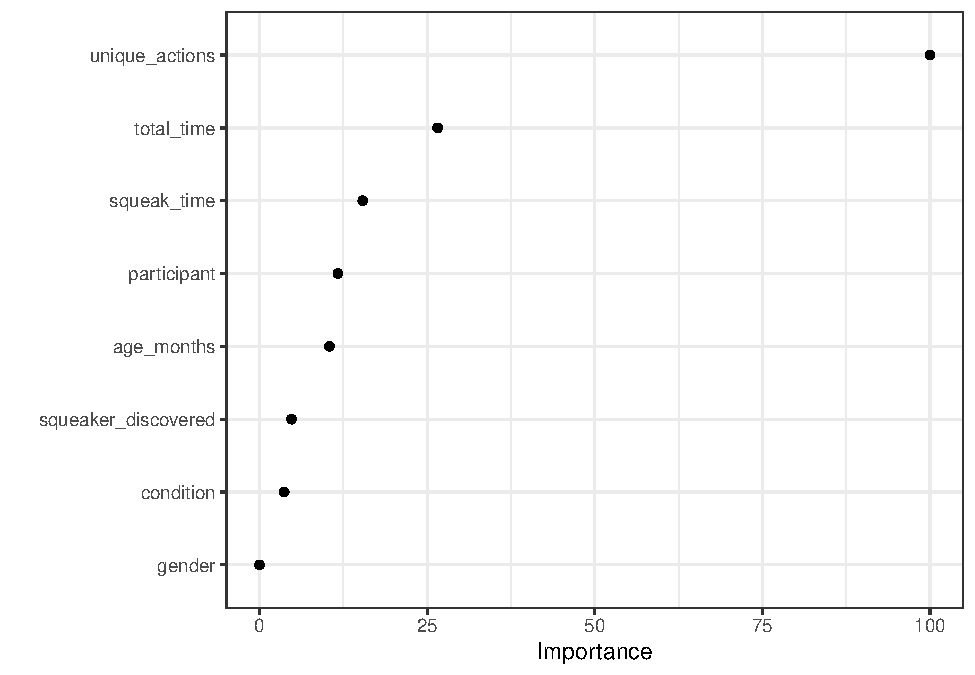
\includegraphics{capstone640_files/figure-latex/unnamed-chunk-5-2.pdf}

\begin{Shaded}
\begin{Highlighting}[]
\NormalTok{coefs }\OtherTok{\textless{}{-}} \FunctionTok{coef}\NormalTok{(ridge}\SpecialCharTok{$}\NormalTok{finalModel,ridge}\SpecialCharTok{$}\NormalTok{bestTune}\SpecialCharTok{$}\NormalTok{lambda)}

\NormalTok{ind   }\OtherTok{\textless{}{-}} \FunctionTok{order}\NormalTok{(}\FunctionTok{abs}\NormalTok{(coefs),}\AttributeTok{decreasing=}\NormalTok{T)}

\CommentTok{\# head(as.matrix(coefs[ind[{-}1],]),10)}
\end{Highlighting}
\end{Shaded}

\hypertarget{results-model-3}{%
\section{Results Model 3}\label{results-model-3}}

In Model 3, we were predicting whether or not a given child discovered the squeaker
`target' function (binary outcome) based upon eight predictors: condition, gender,
total play time, unique actions, time spent playing with the squeaker, number of
target functions discovered, number of total functions discovered, and age in months
(range: 34months-75months). Our results indicated that the model did not capture a
great degree of variance (R-squared = 0.0005), and had a high degree of error (RMSE=
0.83; MAE = 0.67). However, the predictor `unique actions' did seem to be closely
related to the extent to which the squeaker was discovered. Accordingly, the most
important varialbes impacting whether or not the squeaker was discovered were (in
order): number of unique actions, total play time, squeaker play time, participant,
age in months, condition, and gender.

\hypertarget{discussion}{%
\section{Discussion}\label{discussion}}

In terms of descriptives and Model 1, the condition participants were in did not
seem to have an impact on the positive or negative sentiment of their text pedagogy
statements (per Model 1, neither did the function or source type). For the
regularized logistic regression with a categorical outcome in Model 2, the model
didn't seem to capture the predictors behind the rank order results--although in
future, we plan to assess condition variables and child data predictors and drop the
source and function as predictors, since they weren't strongly related to this
outcome. In Model 3, we assessed the degree to which the model capture a binary
child outcome (discovering the squeaker function on the basis of eight predictors).
The strongest related predictor was the number of unique actions a child performed.
This is not altogether unsurprising, since the more actions a child performed on the
toy, the higher their likelihood of discovering the squeaker. In the future, we hope
to delve more deeply into the relations between our naturalistic pedagogy text data
and the text data that is used as an independent pedagogy variable in empirical
studies. That is, do adults accurately create pedagogy types that increase the
likelihood that a child will perform a certain behavior?

\newpage

\hypertarget{references}{%
\section{References}\label{references}}

We used packages from R {[}Version 4.1.1; R Core Team (2021){]} and the R-package \emph{papaja} {[}Version 0.1.0.9997; Aust and Barth (2020){]} for all our analyses.

\begingroup
\setlength{\parindent}{-0.5in}
\setlength{\leftskip}{0.5in}

\hypertarget{refs}{}
\begin{CSLReferences}{1}{0}
\leavevmode\vadjust pre{\hypertarget{ref-R-papaja}{}}%
Aust, F., \& Barth, M. (2020). \emph{{papaja}: {Create} {APA} manuscripts with {R Markdown}}. Retrieved from \url{https://github.com/crsh/papaja}

\leavevmode\vadjust pre{\hypertarget{ref-R-base}{}}%
R Core Team. (2021). \emph{R: A language and environment for statistical computing}. Vienna, Austria: R Foundation for Statistical Computing. Retrieved from \url{https://www.R-project.org/}

\end{CSLReferences}

\endgroup


\end{document}
